\section{\acl{AC1} dan \textit{Acronym3}}

\lipsum[1]

\subsection{\acl{AC1}}

\lipsum[2] To write equation.

\vspace{-12mm}
\begin{flalign}
	\label{eqref1}
	\pi(s,a)^* = argmax(V(s,a)) & &
\end{flalign}
\vspace{-12mm}

For mathematical notation inside text \(\pi\). Reference to figure \ref{imref2}.

\begin{figure}[h]
	\centering
	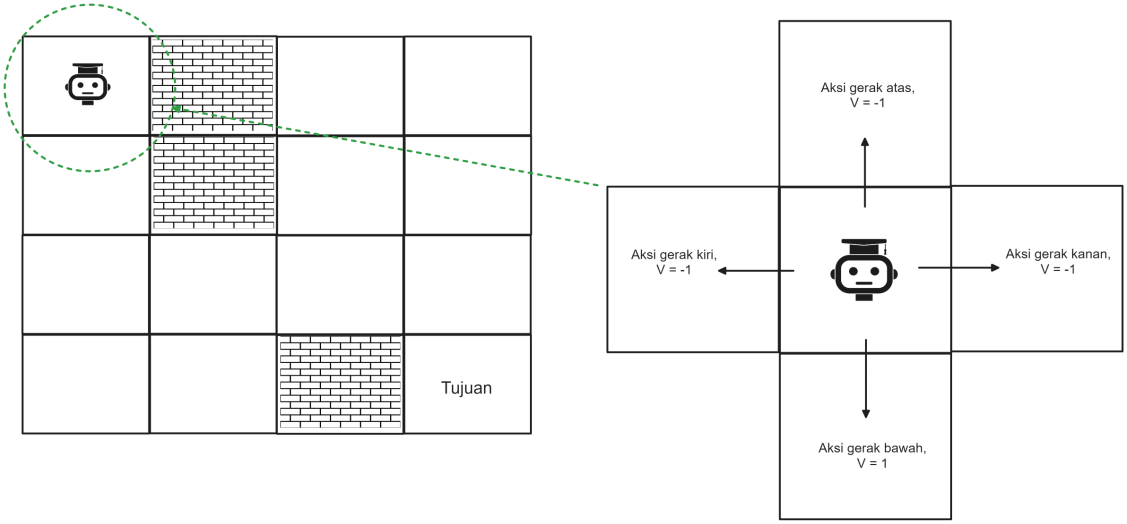
\includegraphics[width=0.8\textwidth]{chapter-2/ilustrasi-RL.png}
	\caption{Second image}
	\label{imref2}
\end{figure}


\subsection{\textit{Acronym3}}

\lipsum[3] Another equation example.

\vspace{-12mm}
\begin{flalign}
	\label{eqref2}
	Q_{new}(s_t,a_t) = (1-\alpha) Q(s_t, a_t) + \alpha (r_t + \gamma \cdot maxQ(s_{t+1},a)) &  &
\end{flalign}
\vspace{-12mm}

Referencing to equation \ref{eqref1}, equation \ref{eqref2}, and figure \ref{imref3}

\begin{figure}[H]
	\centering
	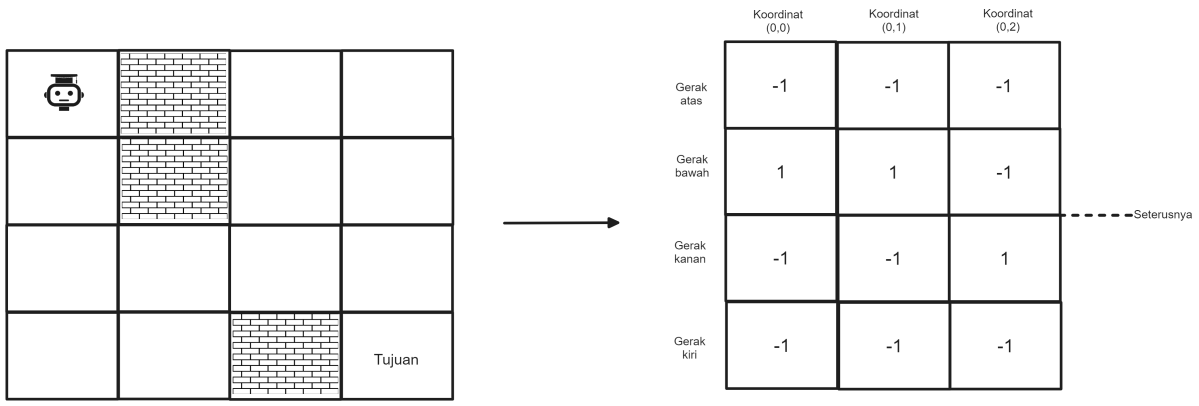
\includegraphics[width=1\textwidth]{chapter-2/ilustrasi-qtable.png}
	\caption{Third image}
	\label{imref3}
\end{figure}


